\section{Github}
\label{sec:Github}
Link for source codes in Lab 4: \href{https://github.com/Lmonk555/lab04_micro_process_control.git}{Link}










\section{Brief Problem}
According to PDF file, we are required to:
\begin{itemize}
    \item Have 4 functions:
    \begin{lstlisting}[language=c]
    // This function will be updated the remaining time of each tasks that are added to a queue. It will be called in the interrupt timer, for example 10 ms.
    void SCH_Update(void)

    // This function will get the task in the queue to run.
    void SCH_Dispatch_Tasks(void)

    // This function is used to add a task to the queue. It should return an ID that is corresponding with the added task.
    uint32_t SCH_Add_Task(void(*pFunction)(),uint32_tDELAY,uint32_tPERIOD):

    // This function is used to delete the task based on its ID.
    uint8_t SCH_Delete_Task(uint32_ttaskID)
    \end{lstlisting}

    \item Must 5 tasks running periodically in 0.5 second, 1 second, 1.5 seconds, 2 seconds, 2.5 seconds.
    \item Add function \texttt{get\_time()} to return the timestamps for every callback of a 10ms tick and 500ms tick.
    \item Do some \texttt{SCH\_Add\_Task()}, make sure the delay is long enough such that the loop is entered before these wake up, print out the current timestamp as each delay expires.
\end{itemize}

\vspace{1em}
And these are unsastified criteria:
\begin{itemize}
    \item Only supporting asingle timeout registered at a time.
    \item Delivering callbacks in the wrong order.
    \item O(n) searches in the \texttt{SCH\_Update} function.
    \item Interrupt frequencies greater than 10Hz, if your timer ticks regularly.
\end{itemize}










\section{Overlay}
In this lab session, we will need 3 files ():
\begin{itemize}
    \item main.c
    \item scheduler.h
    \item scheduler.c
\end{itemize}

However, as we are required to say "no-no" with O(n) in \texttt{SCH\_Update} (which it is in the PDF file), we have to come up with another approach. There are numerous of ways, and we choose to add a function that helps us to arrange the list immediately when adding a new task, which also takes O(n) (but not in \texttt{SCH\_Update}). We do the same to \texttt{SCH\_Delete\_Task} as well.

Therefore, beside the functions that are mandatory, we add 4 extra for the exercise:
\begin{lstlisting}[language=c]
// Return the timestamp for every callback
uint32_t get_time(void);

// Only called by "SCH_Add_Task"
// Get the lastest ID for the added task
static uint32_t Get_New_Task_ID(void)

// Only called by "SCH_Add_Task"
// Insert a task based on Delay, in ascending
static uint32_t Insert(void (*pF)(void), uint32_t delay, uint32_t period, uint32_t id)

// Only called by "SCH_Delete_Task"
// Remove the task at wanted id
static void Remove_At(uint8_t id)
\end{lstlisting}










\section{Functions}
This section only explains what are written in \texttt{scheduler.c}. For more detail, please reach out the \hyperref[sec:Github]{\textcolor{blue}{Github}} source code.

\subsection{Get\_New\_Task\_ID}
Purpose: to get the lastest ID for the adding task, make sure not to handle out "0".
\begin{lstlisting}[language=c]
static uint32_t Get_New_Task_ID(void)
{
    if (++newTaskID == NO_TASK_ID)      // never hand out ID 0
        newTaskID++;
    return newTaskID;
}
\end{lstlisting}



\subsection{SCH\_Init}
Purpose: to initialize the \texttt{SCH\_tasks\_G} array with full of 0 to every \texttt{sTask} struct.

Just called once in \texttt{main.c}.
\begin{lstlisting}[language=c]
void SCH_Init(void)
{
    memset(SCH_tasks_G, 0, sizeof(SCH_tasks_G));
    SCH_count = 0;
    newTaskID = 0;
    tickCount = 0;
    Error_code_G = 0;
}
\end{lstlisting}



\subsection{SCH\_Update}
Purpose: called from the timer ISR every tick. It does NOT run any task, only counts down the head and set \texttt{RunMe} flag.
\begin{lstlisting}[language=c]
void SCH_Update(void)
{
    tickCount++;
    if (SCH_count == 0) return;									// no task in SCH_tasks_G[], return
    if (SCH_tasks_G[0].Delay > 0) SCH_tasks_G[0].Delay--;		// ticks--
    if (SCH_tasks_G[0].Delay == 0) SCH_tasks_G[0].RunMe = 1;	// ticks == 0 --> set it prepare to run
}
\end{lstlisting}



\subsection{Insert}
A sorted \texttt{Insert} itself, only called by \texttt{SCH\_Add\_Task}.

Time Complexity: O(n). Replacing the work for \texttt{SCH\_Update}.
\begin{lstlisting}[language=c]
static uint32_t Insert(void (*pF)(void), uint32_t delay, uint32_t period, uint32_t id)
{
    __disable_irq();
    if (SCH_count >= SCH_MAX_TASKS)             // task list is full
    {
        Error_code_G = ERROR_SCH_TOO_MANY_TASKS;
        __enable_irq();
        return NO_TASK_ID;
    }


    // 1. Find the position by accumulating the delay from SCH_tasks_G[0] and beyond
    uint8_t     idx = 0;
    uint32_t    sum = 0;                        // absolute due time of tasks[idx-1]
    while (idx < SCH_count && sum + SCH_tasks_G[idx].Delay <= delay)
    {
        sum += SCH_tasks_G[idx].Delay;
        idx++;
    }


    // 2. Open a gap for satisfactory Delay slot by shifting the after tasks to the right
    for (uint8_t i = SCH_count; i > idx; i--)
        SCH_tasks_G[i] = SCH_tasks_G[i - 1];


    // 3. Add attributes for the new sTask
    SCH_tasks_G[idx].pTask  = pF;
    SCH_tasks_G[idx].Delay  = delay - sum;
    SCH_tasks_G[idx].Period = period;
    SCH_tasks_G[idx].TaskID = id;
    SCH_tasks_G[idx].RunMe  = (idx == 0 && SCH_tasks_G[idx].Delay == 0);


    // 4. Fix the successor's Delay
    if (idx < SCH_count)
        SCH_tasks_G[idx + 1].Delay -= SCH_tasks_G[idx].Delay;
    SCH_count++;
    __enable_irq();
    return id;
}
\end{lstlisting}



\subsection{SCH\_Add\_Task}
Purpose: ...literally, to add tasks
\begin{lstlisting}[language=c]
uint32_t SCH_Add_Task(void (*pFunction)(), uint32_t DELAY, uint32_t PERIOD)
{
    // returns the task ID (NO_TASK_ID if the list is full)
    return Insert(pFunction, DELAY, PERIOD, Get_New_Task_ID());
}
\end{lstlisting}



\subsection{Remove\_At}
Purpose: to remove sTask at required TaskID by setting its attributes to 0. The successor inherits its Delay so the
tasks behind the successor keep their own Delay.

Only called by \texttt{SCH\_Delete\_Task}.
\begin{lstlisting}[language=c]
static void Remove_At(uint8_t id)
{
    if (id + 1 < SCH_count)
    {
        SCH_tasks_G[id + 1].Delay += SCH_tasks_G[id].Delay;
        SCH_tasks_G[id + 1].RunMe = (id == 0 && SCH_tasks_G[id + 1].Delay == 0);
    }
    for (uint8_t j = id; j + 1 < SCH_count; j++)
        SCH_tasks_G[j] = SCH_tasks_G[j + 1];
    SCH_count--;
    memset(&SCH_tasks_G[SCH_count], 0, sizeof(sTask));
}
\end{lstlisting}



\subsection{SCH\_Delete\_Task}
Purpose: remove required sTask, return Error\_code if needed

Time Complexity: O(n)
\begin{lstlisting}[language=c]
uint8_t SCH_Delete_Task(uint32_t taskID)
{
    uint8_t Return_code = RETURN_ERROR;
    if (taskID != NO_TASK_ID)
    {
        __disable_irq();
        for (uint8_t i = 0; i < SCH_count; i++)
        {
            if (SCH_tasks_G[i].TaskID == taskID)
            {
                Remove_At(i);
                Return_code = RETURN_NORMAL;
                break;
            }
        }
        __enable_irq();
    }
    if (Return_code == RETURN_ERROR)
    {
        Error_code_G = ERROR_SCH_CANNOT_DELETE_TASK;    // no such task
    }
    return Return_code;
}
\end{lstlisting}



\subsection{SCH\_Dispatch\_Tasks}
Purpose: to run the task at ID = 0 when \texttt{RunMe} == 1, check if it's periodic or one-shot to put it back in the list again
\begin{lstlisting}[language=c]
void SCH_Dispatch_Tasks(void)
{
    // Run task when RunMe == 1
    while (SCH_count > 0 && SCH_tasks_G[0].RunMe)
    {
        sTask t = SCH_tasks_G[0];							// copy: the list may change
        __disable_irq();
        Remove_At(0);										// take it out of the list
        __enable_irq();


        // Periodic tasks run again
        // counting while the task runs and a task may delete itself.
        if (t.Period > 0)
            Insert(t.pTask, t.Period, t.Period, t.TaskID);  // put periodic tasks back to the list
        (*t.pTask)();										// run the task
    }
}
\end{lstlisting}



\subsection{get\_time}
Purpose: return timestamp, in \texttt{ms}.
\begin{lstlisting}[language=c]
uint32_t get_time(void)
{
    return tickCount * TICK_MS;
}
\end{lstlisting}










\section{Implementation}
\subsection{Proteus 8}
In order to display the timeout callback, we can either use a terminal or keep it basic with LEDs. For this exercise, we will use a Virtual Machine that can be found in the \texttt{INSTRUMENTS} menu on the left-side bar, or by right-clicking and selecting \texttt{Place -> Virtual Instrument -> VIRTUAL TERMINAL}.

Then, we connect pin PA9 to RXD. This is mandatory, as we will set it up in STM32CubeIDE later.
\begin{figure}[H] 
    \centering 
    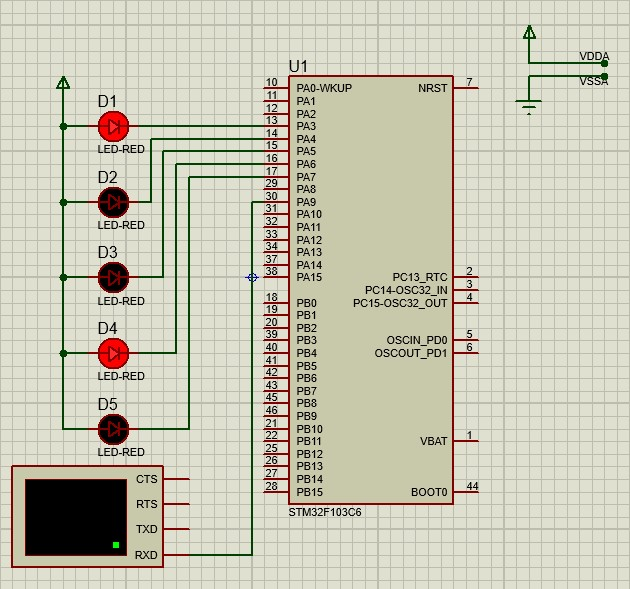
\includegraphics[width=0.8\textwidth]{pictures/schematic.jpg} 
    \caption{Proteus 8 schematic} 
\end{figure}



\subsection{STM32CubeIDE}
For STM32CubeIDE layout, you can use any pin on your choice, but NOT on PA9 and PA10 as we set up USART1 for the Virtual Terminal.
\begin{figure}[H] 
    \centering 
    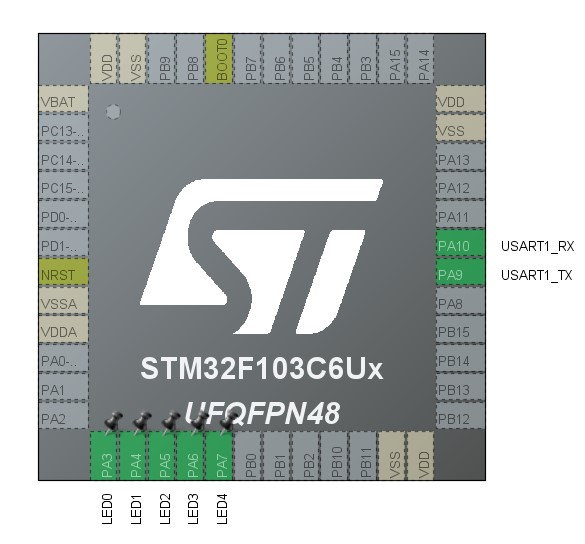
\includegraphics[width=0.7\textwidth]{pictures/stm32cubeide.jpg} 
    \caption{Proteus 8 schematic} 
\end{figure}

\vspace{1em}
Now, for the chip configuration:
\begin{itemize}
    \item Set up the timer TIM2 as previous labs.
    \item Switch to Connectivity categories -> Click USART1 (the program will draw the pin automatically).
    \item In Mode tab:
    \begin{itemize}
        \item Mode: Asynchronous
        \item Hardware Flow Control (RS232): Disable
    \end{itemize}
    \item In Configuration tab -> Parameter Settings:
    \begin{itemize}
        \item Baud Rate: 115200 Bits/s
        \item Word Length: 8 Bits (including Parity)
        \item Parity: None
        \item Stop Bits: 1
    \end{itemize}
\end{itemize}
\begin{figure}[H] 
    \centering 
    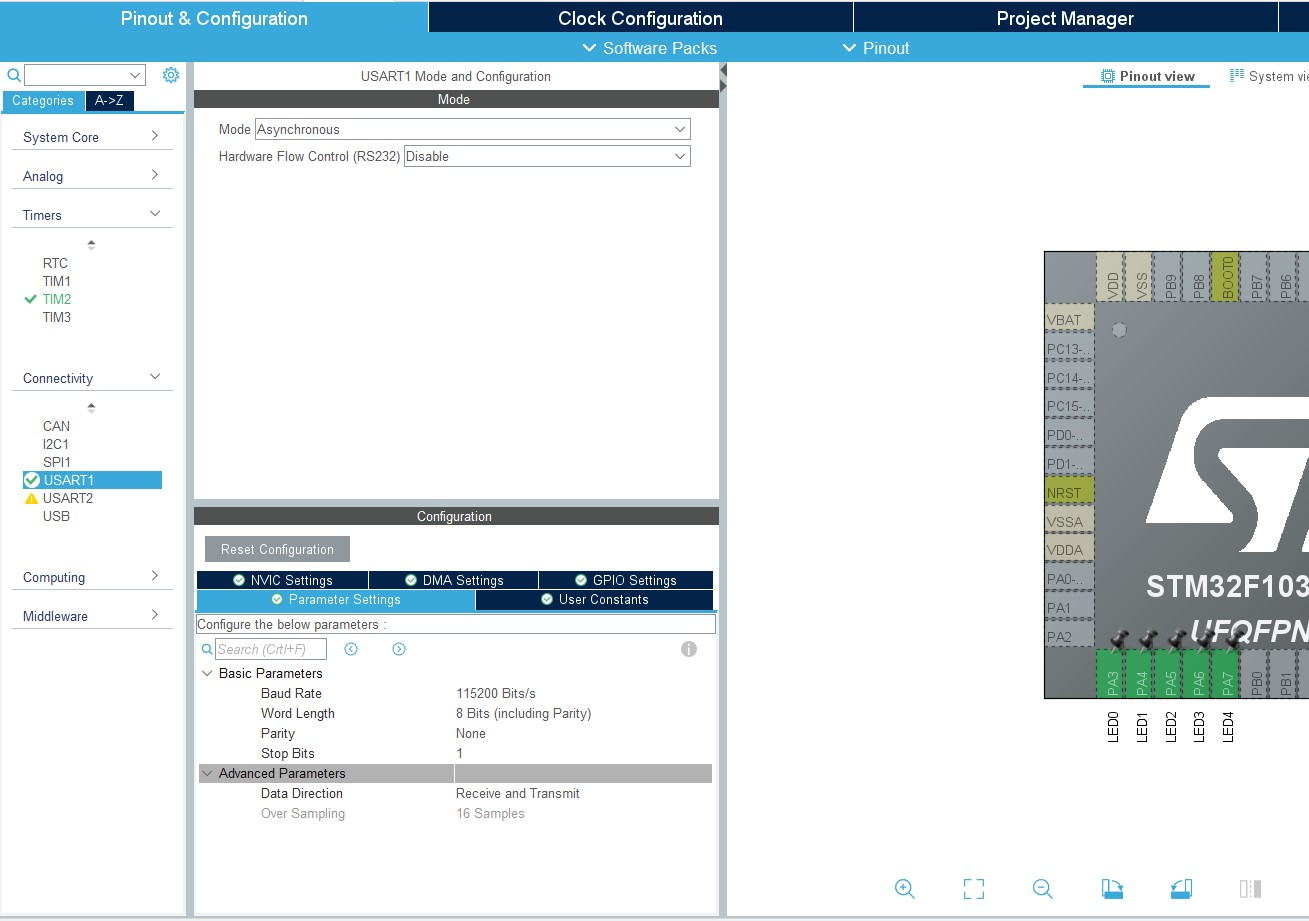
\includegraphics[width=1.0\textwidth]{pictures/usart1.jpg} 
    \caption{Add USART1 configuration} 
\end{figure}

\vspace{1em}
\begin{tcolorbox}
[ 
    colback=white,
    colframe=red!70!black,
    title=Note:,
    colbacktitle=red!70!black,
    coltitle=white,
    fonttitle=\bfseries
]
While implementing, we realized that Proteus8 somehow conflicted with the timer in STM32CubeIDE, which made the tasks went earlier than expected, and it kept sooner and sooner, scaling with the Delay of the task. If you meet the same problem while stimulating in Proteus8, please change Counter Period to 10.
\end{tcolorbox}



\subsection{Code Setup}
These codes are implemented in \texttt{main.c}, you can make your own test based on the format of these codes.
\begin{lstlisting}[language=c, caption=Includes and initialization]
/* Includes ---------------------------*/
#include "main.h"
#include "scheduler.h"
#include <stdio.h>

// Whatever in between, keep as it is

/* USER CODE BEGIN 0 */
void Task0(void) { HAL_GPIO_TogglePin(LED0_GPIO_Port, LED0_Pin); }	// 0.5 s
void Task1(void) { HAL_GPIO_TogglePin(LED1_GPIO_Port, LED1_Pin); }	// 1 s
void Task2(void) { HAL_GPIO_TogglePin(LED2_GPIO_Port, LED2_Pin); }	// 1.5 s
void Task3(void) { HAL_GPIO_TogglePin(LED3_GPIO_Port, LED3_Pin); }	// 2 s
void Task4(void) { HAL_GPIO_TogglePin(LED4_GPIO_Port, LED4_Pin); }	// 2.5 s

// Prints a tag and the value of get_time()
void PrintTime(const char *tag)
{
    char buf[40];
    int n = sprintf(buf, "%s t=%lu ms\r\n", tag, (unsigned long)get_time());
    HAL_UART_Transmit(&huart1, (uint8_t *)buf, n, 10);
}

uint32_t id10ms;

void Task10ms(void)   { PrintTime("[10ms ]"); }
void Print500ms(void) { PrintTime("[500ms]"); }
void Print1s(void)    { PrintTime("[1s   ]"); }
void ShotA(void)      { PrintTime("[shot A]"); }
void ShotB(void)      { PrintTime("[shot B]"); }
void ShotC(void)      { PrintTime("[shot C]"); }
void Stop10ms(void)
{
    SCH_Delete_Task(id10ms);            // demonstrates SCH_Delete_Task
    PrintTime("[10ms stopped]");
}
/* USER CODE END 0 */
\end{lstlisting}


\vspace{1em}
\begin{lstlisting}[language=c, caption=main.c Implementation]
int main(void)
{
    HAL_Init();
    SystemClock_Config();

    /* Initialize all configured peripherals */
    MX_TIM2_Init();
    MX_GPIO_Init();
    MX_USART1_UART_Init();
    /* USER CODE BEGIN 2 */
    SCH_Init();

    // 1 tick = 10 ms --> 50 = 0.5 s, 100 = 1 s,...and so on.
    SCH_Add_Task(Task0, 0, 50);
    SCH_Add_Task(Task1, 1, 100);
    SCH_Add_Task(Task2, 2, 150);
    SCH_Add_Task(Task3, 3, 200);
    SCH_Add_Task(Task4, 4, 250);

    // periodic callbacks that print the time
    id10ms = SCH_Add_Task(Task10ms, 5, 1);  // every 10 ms
    SCH_Add_Task(Print500ms, 7, 50);		// every 500 ms
    SCH_Add_Task(Print1s, 9, 100);			// every 1s (a different interval, running concurrently)
    SCH_Add_Task(Stop10ms, 200, 0);			// at 2s: delete the 10 ms task

    // one-shots
    SCH_Add_Task(ShotA, 300, 0);			// 3 s
    SCH_Add_Task(ShotB, 500, 0);			// 5 s
    SCH_Add_Task(ShotC, 800, 0);			// 8 s

    HAL_TIM_Base_Start_IT(&htim2);
    /* USER CODE END 2 */

    while (1)
    {
        SCH_Dispatch_Tasks();
    }
}
\end{lstlisting}


\vspace{1em}
\begin{lstlisting}[language=c, caption=Other necessary codes]
/* USER CODE BEGIN 4 */
void HAL_TIM_PeriodElapsedCallback(TIM_HandleTypeDef *htim)
{
    if (htim->Instance == TIM2)
        SCH_Update();
}
/* USER CODE END 4 */
\end{lstlisting}





















